% This is auto-generated file: do not edit!
% Exported from microMathematics, version 1.18


Dieses Beispiel demonstriert, wie man
die graphische Darstellung einer
Funktion vorbereitet und anpasst.
Nehmen wir an, wir wollen folgende
Funktion aufzeichnen:
\begin{center}\begin{tabular}{c}
  $f(x) := 25 + 10 \cdot sin \left( \sqrt{ \left| x \right| } \right) $
\end{tabular}\end{center}

Das Funktionsargument, das die x-Werte
repräsentiert, wird für N Punkte
innerhalb des Intervalls [x1, x2]
eingesetzt:
\begin{center}\begin{tabular}{ccc}
  $N := 300$ &
  $x1 := -30$ &
  $x2 := 30$ \cr
\end{tabular}\end{center}
\begin{center}\begin{tabular}{c}
  $x := \left[ x1,\, x1 + \left( x2 - x1 \right) / N \,..\, x2 \right]$
\end{tabular}\end{center}

Ist die Funktion und das Argument
definiert, können Sie die Plot Box
hinzufügen indem Sie den ''Neu'' Button
der Menüleiste oder den
''Funktionsgraph hinzufügen'' Button in
der Werkzeugleiste wählen:
\begin{center}\begin{tabular}{c} 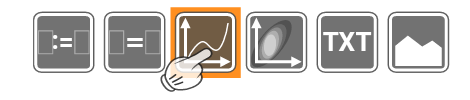
\includegraphics[resolution=320]{graphics/function_plot_fig1.png} \end{tabular}\end{center}
\begin{center}\begin{tabular}{c} 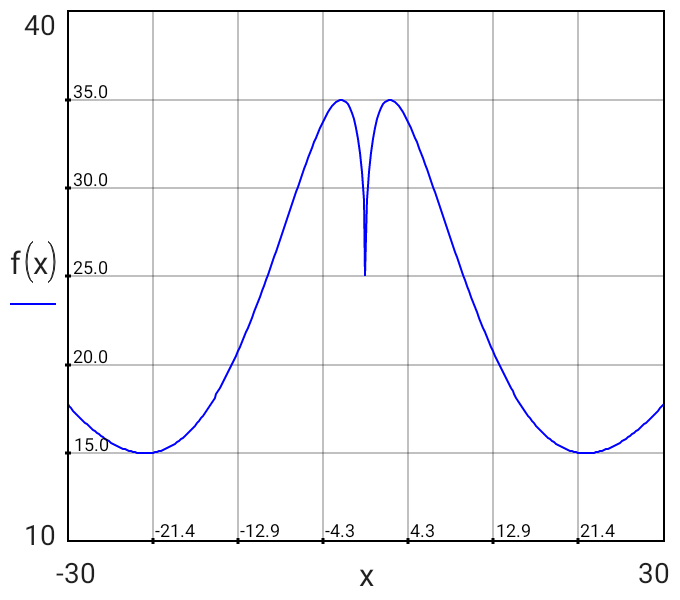
\includegraphics[resolution=320]{graphics/function_plot_fig2.png} \end{tabular}\end{center}

Die darzustellende Funktion soll ins
linke Mittelfeld eingefügt werden. Es
kann ebenfalls eine integrierte oder
zuvor definierte Funktion sein sowie
ein mathematischer Ausdruck, der jeden
anderen Operator oder Funktion
enthalten kann.

Das Funktionsargument, das die x-Werte
repräsentiert, wird in das untere
Mittelfeld eingesetzt. Dies kann eine
Variable eines Intervalltyps oder ein
mathematischer Ausdruck sein, der eine
Intervallvariable enthält.

Die vier anderen Felder definieren die
Plot Grenzen. Falls diese Elemente
leer bleiben, wird das Programm die
entsprechenden Werte automatisch
berechnen. Allerdings können Sie diese
Felder zu jedem Zeitpunkt bearbeiten
und die Werte einsetzten, die Sie
benötigen.

Wenn Sie lange auf die Mitte des Plot
Bereichs drücken, ein Action Button
''Objekteinstellungen'' erscheint:
\begin{center}\begin{tabular}{c} 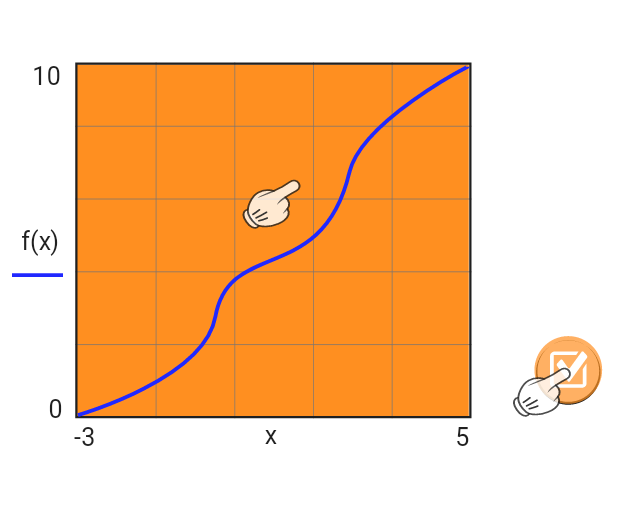
\includegraphics[resolution=320]{graphics/function_plot_fig3.png} \end{tabular}\end{center}

Ein Tap auf diesen Button öffnet das
Dialogfenster ''Plot Einstellungen''.
Hier können die Größe und das Aussehen
des Graphen verändert werden. Ein
verschränkter Graph sieht
beispielsweise so aus:
\begin{center}\begin{tabular}{c} 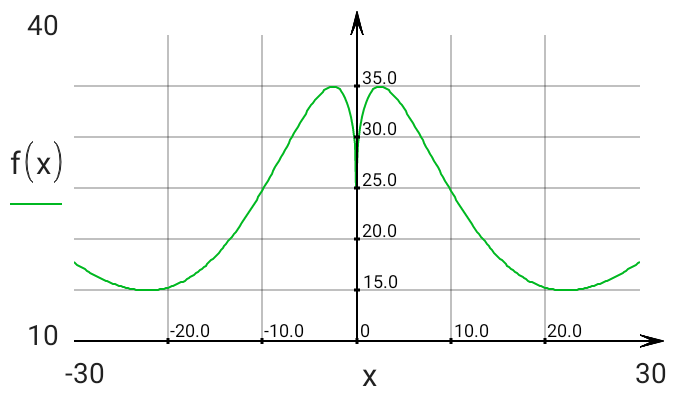
\includegraphics[resolution=320]{graphics/function_plot_fig4.png} \end{tabular}\end{center}

Sie können Strichfarbe, -weite und
-stil im ''Stricheinstellungen'' Dialog
ändern. Es erscheint zudem, wenn Sie
lange auf den grünen Marker unterhalb
des Funktionsnamens auf der linken
Seite des Plot Bereiches drücken:
\begin{center}\begin{tabular}{c} 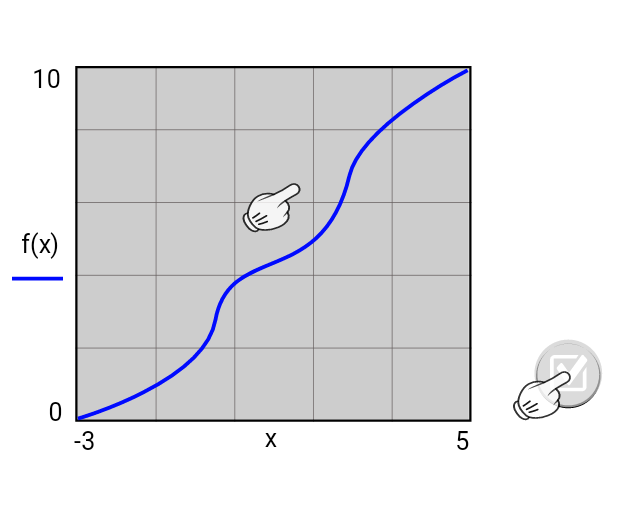
\includegraphics[resolution=320]{graphics/function_plot_fig5.png} \end{tabular}\end{center}

Zum Beispiel, man kann gestrichelte
Linien benutzen:
\begin{center}\begin{tabular}{c} 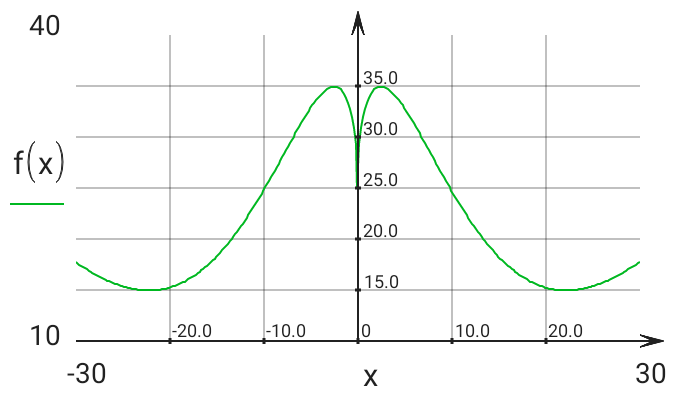
\includegraphics[resolution=320]{graphics/function_plot_fig6.png} \end{tabular}\end{center}

Die Anzahl von Achsenbezeichnungen und
Rasterlinienfarben kann in den
''Rastereinstellungen'' Dialog verändert
werden. Es erscheint, wenn Sie lange
auf den Freiraum zwischen dem
minimalem x-Wert (-30) und dem
Argumentsymbol (x) oder zwischen das
x-Symbol und den maximalen x-Wert (30)
unterhalb des Plot Bereichs drücken:
\begin{center}\begin{tabular}{c} 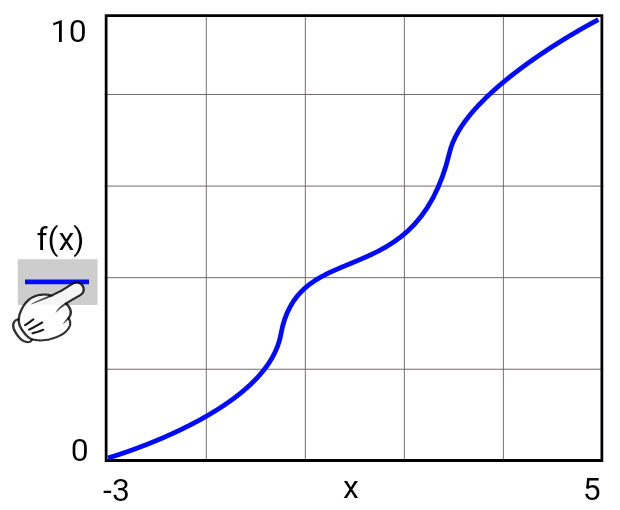
\includegraphics[resolution=320]{graphics/function_plot_fig7.png} \end{tabular}\end{center}
\begin{center}\begin{tabular}{c} 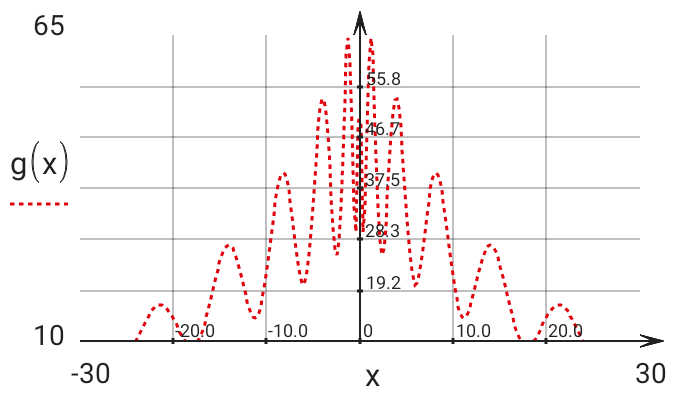
\includegraphics[resolution=320]{graphics/function_plot_fig8.png} \end{tabular}\end{center}